\documentclass{article}
\usepackage[utf8]{inputenc}

\title{IF683 -PROJETO DE DESENVOLVIMENTO}
\author{erbert.gadelha }
\date{Maio 2019}

\usepackage{natbib}
\usepackage{graphicx}
\usepackage{enumerate}
\usepackage{float}
\usepackage{url}
\usepackage{hyperref}

\begin{document}

\maketitle

\section{Introdução}
	O Projeto de desenvolvimento (Projetão) trata-se de uma matéria que dá espaço aos universitários para que desenvolvam projetos dentro da universidade com o auxílio da própria instituição.

\begin{figure}[h!]
    \centering
    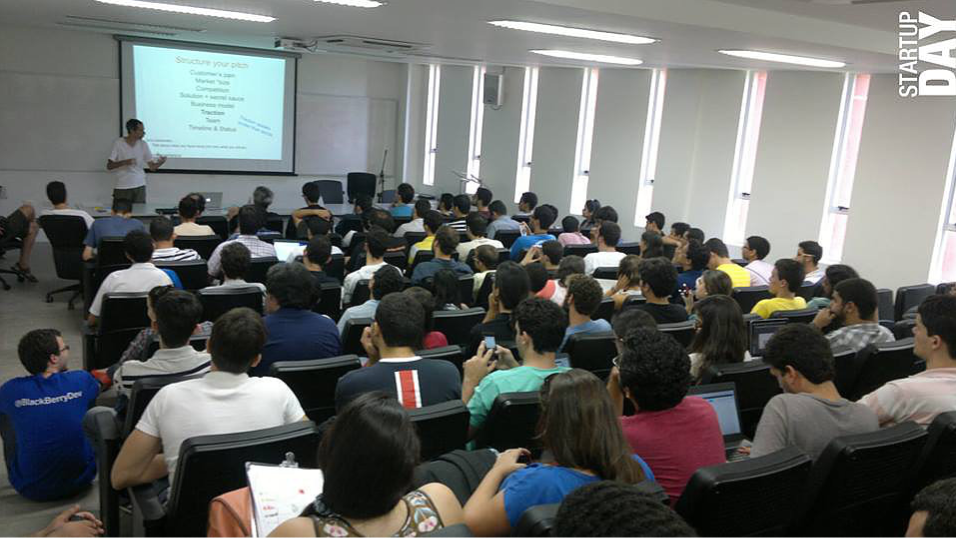
\includegraphics[scale=0.3]{imagem_01.jpg}
    \caption{Alunos recebendo dicas e orientações quanto ao desenvolvimento de projetos.}
    \label{fig:imagem_01.jpg}
\end{figure}

Abaixo será exibido pequenos resumos dos que são dados pela matéria. (Os assuntos da matéria podem ser encontrados no site \cite{ref_aulas}) 

\begin{table}[h]
    \centering
    \begin{tabular}{c|l}
        \hline
        Construção de&O desenvolvimento de uma persona é uma prática que agiliza\\Personas&e torna mais coerente o desenvolvimento de um projeto.\\&Por isso, vem a ser um conhecimento essencial para área.\\
        \hline
        Pitch&Pitch trata-se de uma forma de apresentar seu projeto/ideia\\&de forma ágil e direta. Portanto, é importantíssimo o domínio\\&de apresentações em pitch caso você queira conquistar apoiadores\\&e/ou clientes para o seu projeto.\\
        \hline
    \end{tabular}
    \label{tab:my_label}
\end{table}

\section{Relevância}
	Por se basear no desenvolvimento de projetos, o curso acaba por estimular boas praticas para os alunos, além de muitas vezes ser o primeiro passo deles na carreira, dando a eles também uma melhor visão de sua carreira.

\begin{figure}[h!]
    \centering
    
\includegraphics[scale=0.3]{imagem_02.jpg}
    \caption{Projetos que estão sendo desenvolvidos atualmente.}
    \label{fig:imagem_02.jpg}
\end{figure}

\begin{table}[h]
    \centering
    \begin{tabular}{c|l}
        Projeto&Descrição\\
        \hline
        Cote Aqui \cite{ref_coteaqui}&Trata-se de um catálogo online com foco na venda de materiais\\&de construção.
    \end{tabular}
    \label{tab:my_label}
\end{table}

\section{Relação com outras disciplinas}
	Para o desenvolvimento dos projetos, os alunos deverão utilizar os conhecimentos adquiridos nos anos anteriores de curso. Por isso todo o embasamento adquirido durante o curso faz-se necessário.

\bibliographystyle{plain}
\bibliography{referencias}


\end{document}
